\section{Aufbau}
\label{sec:Aufbau}
Die zylinderförmige $\ce{KBr}$-Probe befindet sich auf einer Metallplatte,
die als eine der Kondensatorplatten dient, die andere Kondensatorplatte
liegt auf der Probe. Von der unteren Platte aus geht ein Metallstab runter,
dieser wird in ein mit flüßigem Stickstoff gefülltes Dewar-Gefäß gefahren,
um die Probe kühlen zu können.
Die Probe befindet sich in einer Kammer, welche bis auf
$\SI{e-2}{\milli\bar}$ %$\SI{20}{\milli\bar}$
evakuiert ist. Dies ist notwendig, da die Probe hygroskopisch ist.
Außerhalb der Kammer der Probe befindet sich eine Heizvorrichtung
zur Temperaturregelung.

Eine schematische Skizze des Aufbaus ist in Abbildung \ref{fig:skizze} zu sehen.

\section{Durchführung}
\label{sec:durchfuehrung}
Die Probe wird auf eine Temperatur von $T = \SI{320}{\kelvin}$ aufgeheizt
und an die Platten die Spannung $U = \SI{900}{\volt}$ angelegt
und für $\SI{900}{\second}$ aufrecht erhalten. Dann wird die Probe mit
flüßigem Stickstoff auf $T = -\SI{45}{\celsius}$ abgekühlt und in zwei
Messreihen mit unterschiedlichen konstanten Heizraten erwärmt.
Es werden in regelmäßigen Zeitabständen Messwerte für den
Depolarisationsstrom und die Temperatur notiert.
Bei der größeren Heizrate alle $\SI{30}{\second}$, bei der kleineren jede Minute.

\begin{figure}
    \centering
    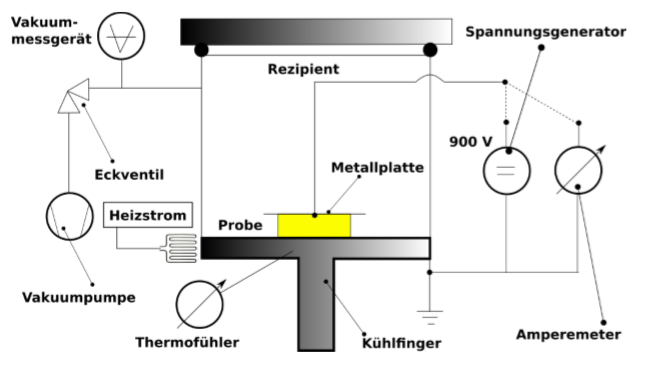
\includegraphics[width=0.8\textwidth]{pdf/aufbauSkizze.png}
    \caption{Schematische Skizze des verwendeten Aufbaus \cite{anleitung}.}
    \label{fig:skizze}
\end{figure}
